\section{Atoms in optical cavities}

In cavity quantum electrodynamics (cavity QED) there are cases where the spontaneous emission of the atoms is essential. It's possible, however, to suppress the spontaneous emission if we detune the laser far from the atomic resonance frequency. In that case coherent scattering of the photons are dominant and there's a significant optical dipole force. Due to the confinement of the cavity, the back-action of the atoms onto the laser becomes significant, whereas it's negligible in free space.

\section{Types of optical cavities}
There are different types of cavities, such as the bow-tie, the ring and the Fabry-Perot cavity. In the case of the Fabry-Perot cavity, there are two curved mirrors separated by a distance $d$. If $d = n \lambda / 2$, the system is in resonance and there's a strong light field in the cavity. Thus boundary conditions on light space determine the modes of the frequency space.

\section{The Jaynes-Cummings Hamiltonian}
The Jaynes-Cummings model describes the interaction of a two-level atom with a single mode of a cavity field \cite{jaynes}. The Jaynes-Cummings Hamiltonian is:

\begin{align}
\begin{split}
H_\text{JC} = \underbrace{p^2 / 2m}_\text{atom} + \underbrace{V_\text{ext}(x)}_\text{external potential} - \underbrace{1/2 \hbar \omega_\text{a} \sigma_z}_\text{atomic transitions} - \underbrace{\hbar \omega_\text{c} a^\dagger a}_\text{field} + \underbrace{\hbar \eta (a e^{i \omega_\text{l} t} + a^\dagger e^{-i \omega_\text{l} t})}_\text{pumping} + \\
+ \underbrace{\hbar g_0 \cos(kx) (\sigma^+ a + \sigma^- a^\dagger)}_\text{field-atom interaction},
\end{split}
\end{align}where $\omega_\text{a}$ is the resonance frequency of the atom, $\sigma_z$ the Pauli spin matrix, $\omega_\text{c}$, the resonance frequency of the cavity, $a^\dagger$ and $a$ the creation and annihilation operators, $\eta$ the pumping strength, $\omega_\text{l}$ the frequency of the laser, $U_0$ the coupling constant and $\sigma^+$ and $\sigma^-$ the raising and lowering operators. A detailed derivation of the Jaynes-Cummings Hamiltonian can be found at \cite{collapseandrevival}. In order to get rid of the explicit time-dependence, we transform the Hamiltonian to a frame rotating with $\omega_\text{l}$. The Hamiltonian now reads:

\begin{align}
\begin{split}
H_\text{JC} = \frac{p^2}{2m} + V_\text{ext}(x) - \hbar \Delta_\text{a} \sigma_z - \hbar \Delta_\text{c} a^\dagger a + \hbar \eta (a + a^\dagger) + \\
+ \hbar g_0 \cos(kx) (\sigma^+ a + \sigma^- a^\dagger),
\end{split}
\end{align}where $\Delta_\text{a} = \omega_\text{l} - \omega_\text{a}$ and $\Delta_\text{c} = \omega_\text{l} - \omega_\text{c}$.

\section{Detuning}
In our case, the pumping laser is far detuned from the atomic resonance frequency, i.e. $\Delta_\text{a} = \omega_\text{l} - \omega_\text{a}$ is large. Thus the excitation probability of the atom is vanishing and we neglect the $\sigma_z$-term. Now we derive heuristically a modified Hamiltonian. Going to the Heisenberg picture:

\begin{align}
\dot{a} = \frac{i}{\hbar} [H, a] = i \Delta_\text{c} a - i \eta -i g_0 \cos(kx) \sigma^-.
\end{align}The time-derivative for the raising operator reads:

\begin{align}
\dot{\sigma}^+ = -i \Delta_\text{a} \sigma^+ + i g_0 \cos(kx) a^\dagger.
\end{align}We're not interested in fast dynamics, so we set $\dot{\sigma}^+ = 0$. We obtain

\begin{align}
\sigma^+ = \frac{g_0 }{\Delta_\text{a}} \cos(kx) a^\dagger && \sigma^- = \frac{g_0 }{\Delta_\text{a}} \cos(kx) a.
\end{align}We obtain:

\begin{align}
\dot{a} = -i \Delta_\text{c} a + \frac{i g_0}{\Delta_\text{a}}  \cos(kx) a - i \eta.
\end{align}We can thus make a guess of the effective Hamiltonian:

\begin{align}
H = \frac{p^2}{2m} = V_\text{ext}(x) - \hbar \Delta_\text{c} a^\dagger a + \hbar \eta (a + a^\dagger) + \hbar U_0 \cos(kx)^2,
\end{align}where we set $U_0 \coloneqq g_0^2 / \Delta_\text{a}$.

\section{Transversal Pump}

Now we want to focus our attention at a different case where the laser is incident transversally relative to the axis of the mirrors. The cavity mode will thus only be populated by photons which were scattered off the atoms. The Hamiltonian now reads:

\begin{align}
\begin{split}
H_\text{trans} = \frac{p^2}{2m} + V_\text{ext}(x) - \hbar \Delta_\text{c} a^\dagger a  + \hbar \eta \cos(kx) \cos(kz) (a + a^\dagger) + \\
+ \hbar \frac{\Omega^2}{\Delta_\text{a}} \cos(kz)^2 + \hbar U_0 \cos(kx)^2 a^\dagger a,
\end{split}
\end{align}where $\Omega$ is the Rabi frequency. Now we get an an effective long-range atom-atom interaction. The periodicity of the potential which is destructive for $\lambda / 2$ and constructive for $\lambda$. The atoms either minimize energy by being homogeneously distributed or by being localized at local potential minima. With the pump strength $\eta$ we control which configuration the atoms "choose". We define an \textit{order parameter} $\Theta$, which indicates whether the atoms are uniformly distributed or localized at potential minima:

\begin{align}
\Theta \coloneqq \langle \psi | \cos(kx) | \psi \rangle.
\end{align}At $\Theta = 0$, there's a uniform distribution and at $\Theta = \pm 1$, the atoms are localized at even or odd antinodes. An analytic solution of $\Theta$ and the lattice potential can be seen in Figure~\ref{fig:self-organization}.

\begin{figure}[!htb]
	\begin{minipage}[b]{.5\linewidth}
	\centering
	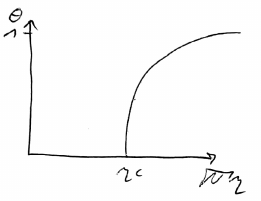
\includegraphics[width=1\linewidth]{images/order_parameter.png}
	\subcaption{Order parameter.}
	\end{minipage}
%
	\begin{minipage}[b]{.5\linewidth}
	\centering
	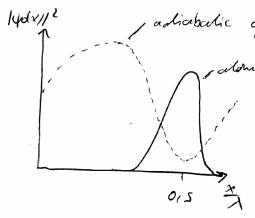
\includegraphics[width=1\linewidth]{images/lattice_potential.png}
	\subcaption{Lattice potential.}
	\end{minipage}
\caption{Order parameter and lattice potential.}
\label{fig:self-organization}
\end{figure}
\FloatBarrier